% !TEX root = ../main.tex
Конвейер нужен, чтобы детектор из главы~2 видел один и тот же вектор признаков и на публичном бенчмарке, и на метрике своего приложения.
Реализация~--- модульный ETL на Python~3.12.
Сырой файл остаётся в каталоге RAW, нормализованный кадр~--- в PROCESSED, итоговый набор~--- в UNIFIED.
Повторный запуск читает сырьё заново и не правит его.

\section{Источники и их роли}

В работе четыре источника.
Путать их в одной матрице нельзя: у них разные роли, и модель учится внутри одного ряда \((\texttt{source},\texttt{service},\texttt{metric\_name})\).

\begin{table}[ht]
\centering
\begin{tabular}{llp{7.2cm}}
\toprule
Источник & Метки & Роль \\
\midrule
NAB \cite{numenta-nab} & окна \(0/1\) & публичный бенчмарк \\
KPI \cite{kpi-ad} & метки организаторов \(0/1\) & основная количественная оценка \\
Prometheus \cite{prometheus} & нет (\(-1\)) & телеметрия приложения и инфраструктуры \\
Zabbix \cite{zabbix} & нет (\(-1\)) & телеметрия тестового контура \\
\bottomrule
\end{tabular}
\caption{Роли источников данных.}
\end{table}

\subsection{NAB}

Numenta Anomaly Benchmark~--- набор одномерных рядов: температура оборудования, загрузка процессора, объёмы обращений, искусственные сигналы с заранее нарисованной аномалией.
Каждый ряд лежит отдельным CSV.
Метка точки равна \(1\), если её время попадает в окно из файла \texttt{combined\_windows.json}, и \(0\) в остальных случаях.
Каталог с окнами загрузчик не читает как ряд.
В прогоне сравнения участвуют 58 CSV.

\subsection{KPI}

KPI Anomaly Detection~--- длинные операторские индикаторы.
Организаторы заранее разделили обучение и проверку: \texttt{phase2\_train.csv.gz} и \texttt{phase2\_ground\_truth.csv.gz}.
Идентификатор ряда~--- поле KPI ID.
В unified оба файла можно склеить, но для оценки модели склейка не используется: глава~2 читает их раздельно и дополнительно отбрасывает из обучения точки, которые не строго раньше первой тестовой метки того же ряда.

\subsection{Prometheus}

Prometheus уже собирает метрики приложения и машин, на которых оно стоит.
В конвейер попадают локальные parquet-дампы из \texttt{datasets/raw/PROMETHEUS/}.
Живой сервер опрашивается только если при запуске явно передан \texttt{--prom-url}.
У серии сохраняется JSON меток \texttt{job}, \texttt{instance}, \texttt{cpu}, \texttt{mode}, чтобы два одноимённых счётчика с разных машин не слиплись в один ряд.
Гистограммные ряды \texttt{*\_bucket} и служебные \texttt{*\_created} в модельный набор не берутся: это не значение сигнала, а сетка гистограммы и время создания ряда.

Годовая выгрузка приложения лежит отдельно от короткого снимка, который вошёл в unified августа 2026~г.
В каталоге \texttt{live} собрано 772 parquet.
Там есть ряды приложения (backend, bot, worker), PostgreSQL, Redis, node-exporter и проверки blackbox.
Хранение на сервере начинается с 4~августа 2026~г.
Метрики хоста берутся из node-exporter.

\subsection{Zabbix}

Zabbix тестового контура снят дампами PostgreSQL и разложен двумя parquet, потому что у истории и у трендов разный шаг.
История, \texttt{zabbix\_history.parquet}, содержит 16\,626\,504 строк.
Имя метрики~--- ключ элемента, поле \texttt{service}~--- имя хоста, метка равна \(-1\).
Тренды, \texttt{zabbix\_trends.parquet}, содержат 14\,380\,893 строк.
К ключу добавлен суффикс \texttt{\{grain="trend\_avg"\}}, значение~--- среднее за интервал тренда.
Смешивать эти два зерна в одном ряде нельзя: скользящее окно из пяти точек означало бы пять минут на истории и пять интервалов тренда на другом файле.

\section{Единая схема}

Каждый загрузчик заканчивает кадр одними и теми же колонками:
\texttt{timestamp}, \texttt{service}, \texttt{metric\_name}, \texttt{value}, \texttt{label}, \texttt{source}.
Метка принимает три значения.
\(0\)~--- норма, \(1\)~--- аномалия, \(-1\)~--- метки нет.
Precision, recall и PR-AUC считаются только по точкам \(0\) и \(1\).

Нормализация приводит время к одному типу, удаляет пустые значения и точные дубликаты и сортирует ряд по времени.
Имена метрик NAB и KPI приводятся к каноническому виду по токенам, чтобы один и тот же показатель не раздвоился из-за регистра или лишнего символа.
Ключи Zabbix и имена Prometheus не переименовываются в условные \texttt{cpu\_usage}: промышленное имя должно остаться тем, по которому оператор найдёт ряд в своей системе.

\section{Модули конвейера}

\begin{itemize}
  \item извлечение~--- \texttt{etl/loaders/}, отдельные загрузчики NAB, KPI, Prometheus и Zabbix;
  \item нормализация~--- \texttt{normalize\_dataframe()};
  \item признаки~--- скользящие статистики и разности внутри ряда;
  \item запись~--- Parquet как основной формат и CSV для просмотра;
  \item запуск~--- \texttt{etl/pipeline.py} и команда \texttt{main.py}.
\end{itemize}

Команды соответствуют источникам: \texttt{nab}, \texttt{kpi}, \texttt{prometheus}, \texttt{zabbix} и общий \texttt{all}.
Общий запуск по умолчанию читает локальные каталоги и не ходит в сеть.
Полный набор живых parquet и оба файла Zabbix в один процесс не склеиваются: такой кадр не помещается в память как единая таблица.
Для оценки моделей они и не нужны единым файлом.
Сравнение в главе~2 читает NAB и срез KPI само, минуя этот общий кадр.

\section{Признаки ряда}

После сортировки по времени для каждой точки считаются восемь признаков:
\texttt{rolling\_mean\_5}, \texttt{rolling\_mean\_15},
\texttt{rolling\_std\_5}, \texttt{rolling\_std\_15},
\texttt{rolling\_min\_5}, \texttt{rolling\_max\_5},
приращение \texttt{delta} и относительное изменение \texttt{percent\_change}.
Окно не переходит границу ряда.
В начале ряда, где истории ещё нет, пропуски признаков заполняются нулём уже в \texttt{ml\_dataset}, чтобы матрица для sklearn была плотной.

В детектор подаются исходное \texttt{value} и эти восемь колонок.
Порог по одной только величине такого вектора не видит: z-score и правило Тьюки в главе~2 специально оставлены на одной колонке \texttt{value}, чтобы было с чем сравнить методы, которые смотрят весь вектор.

\begin{figure}[ht]
\centering
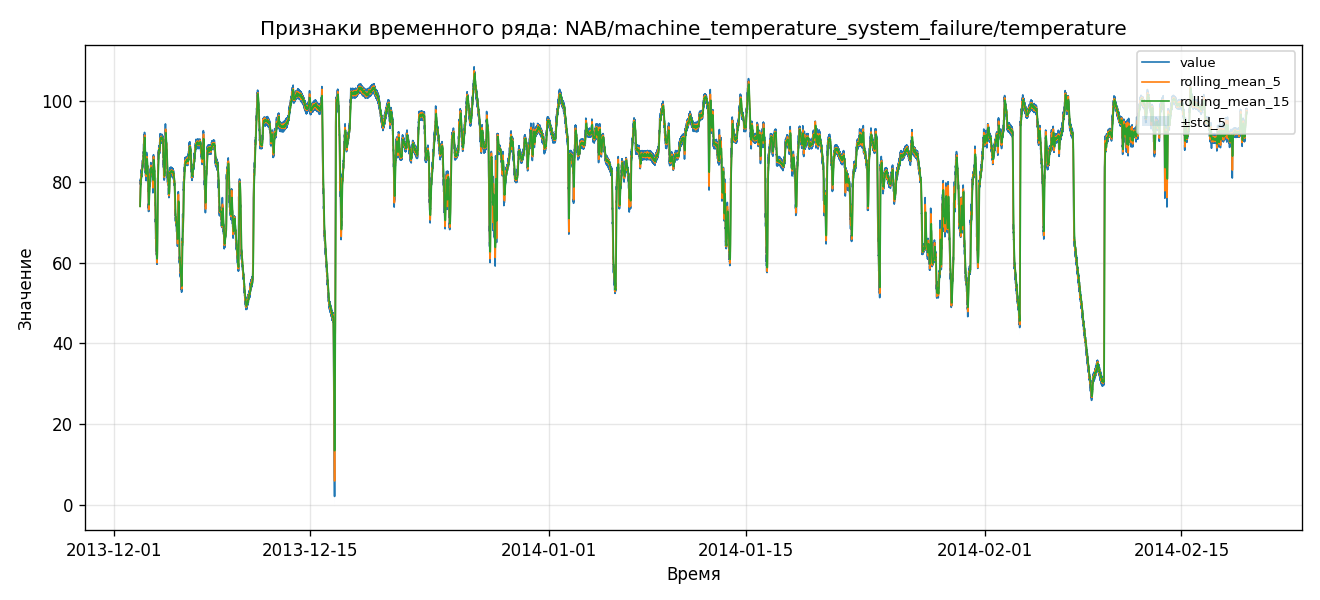
\includegraphics[width=0.92\textwidth]{NAB/features_data.png}
\caption{Ряд температуры из NAB: значение и скользящие признаки. Резкое падение видно и на среднем, и на отклонении.}
\end{figure}

На промышленном счётчике тот же расчёт выглядит иначе.
\texttt{node\_cpu\_seconds\_total} в режиме простоя растёт почти линейно: это накопительный счётчик, а не уровень загрузки.
Само значение тогда мало говорит об аномалии, а \texttt{delta} переводит его в приращение за шаг.

\begin{figure}[ht]
\centering
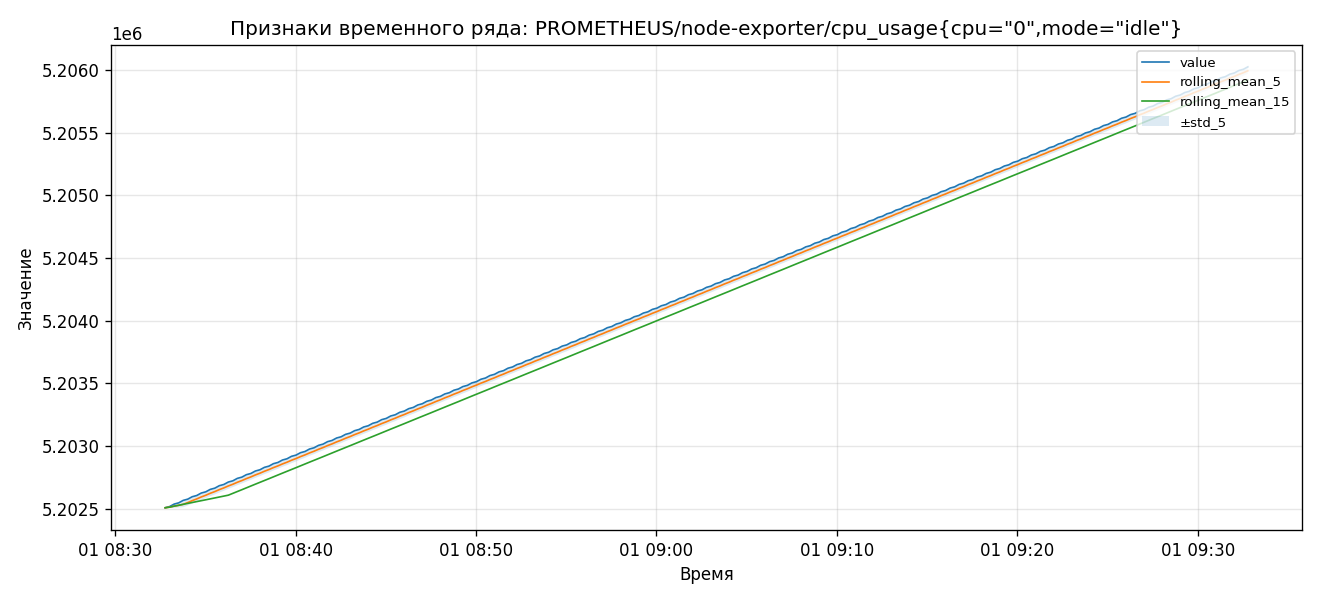
\includegraphics[width=0.92\textwidth]{PROMETHEUS/features_data.png}
\caption{Счётчик простоя CPU из node-exporter. Уровень растёт монотонно, рабочий сигнал для детектора~--- приращение.}
\end{figure}

\FloatBarrier
\section{Состав размеченного набора}

После исправления загрузчиков и привязки окон NAB полный unified-прогон дал следующий состав.
В нём короткий демонстрационный Prometheus.
Годовая выгрузка и Zabbix в этот файл не входили и лежат отдельными parquet.

\begin{table}[ht]
\centering
\begin{tabular}{lrr}
\toprule
Источник & Строк & Аномалий (\(\texttt{label}=1\)) \\
\midrule
NAB & 365\,541 & 33\,495 \\
KPI & 5\,922\,913 & 134\,114 \\
Prometheus & 4\,097 & 0 \\
\midrule
Всего & 6\,292\,551 & --- \\
\bottomrule
\end{tabular}
\caption{Состав unified-набора после исправления конвейера.}
\end{table}

Доля аномалий на NAB около \(9\,\%\), на KPI около \(2\,\%\).
На таком перекосе доля верных ответов почти ничего не говорит: детектор, который всегда отвечает <<норма>>, уже выглядит успешным.
Поэтому в главе~2 главный показатель~--- PR-AUC.

\begin{figure}[ht]
\centering
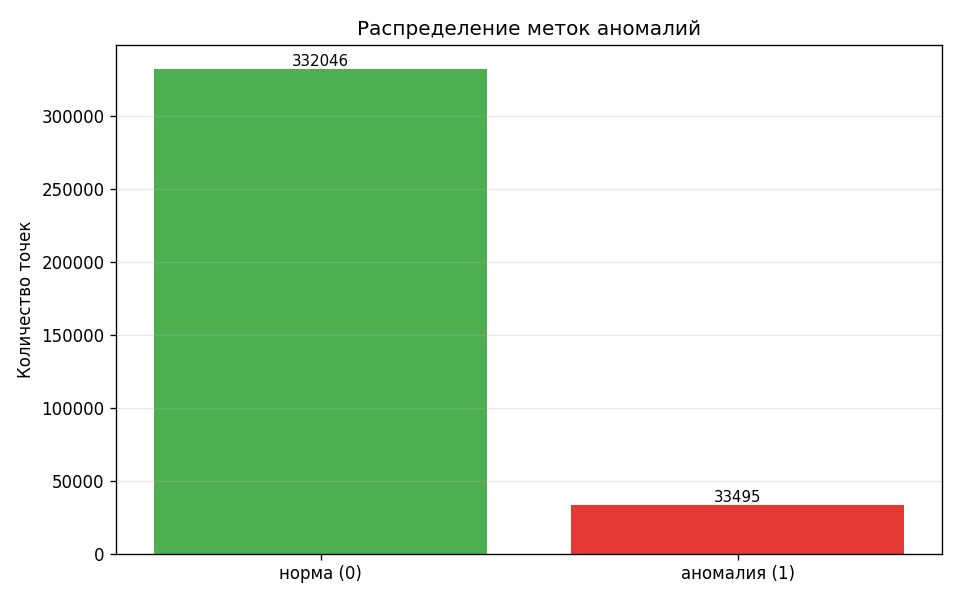
\includegraphics[width=0.78\textwidth]{NAB/anomaly_distribution.png}
\caption{Метки NAB: 332\,046 точек нормы и 33\,495 аномалий.}
\end{figure}

\begin{figure}[ht]
\centering
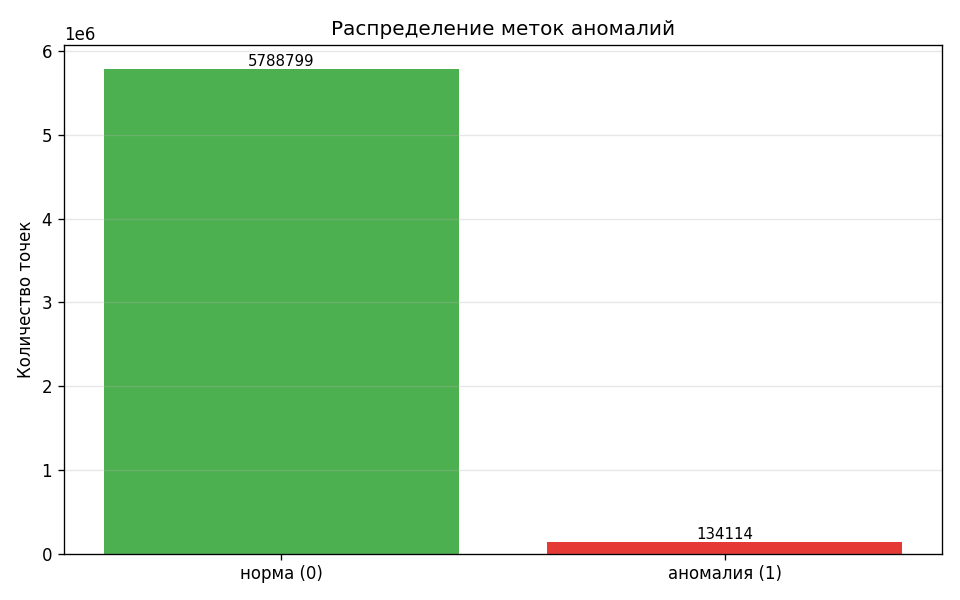
\includegraphics[width=0.78\textwidth]{KPI/anomaly_distribution.png}
\caption{Метки KPI: 5\,788\,799 точек нормы и 134\,114 аномалий.}
\end{figure}

Автотесты проверяют состав колонок, загрузчики, временной разрез и то, что в таблицу сравнения не попадают Prometheus и Zabbix.
Графики прогона конвейера пишутся в \texttt{reports/current/}.
Каталог \texttt{reports/before/} хранит снимок прежнего прогона и текущим кодом не перезаписывается.
Демонстрационный интерфейс \texttt{gui/app.py} показывает схему и уже построенные файлы.
Он не запускает загрузку и не учит модель.

\section{Что не входит в оценку качества}

Prometheus и Zabbix нужны как вход будущего сервиса и как проверка, что тот же код признаков читает промышленный ряд.
Строки качества по ним не считаются: эталона \(0/1\) нет.
Живые выгрузки в публичный репозиторий не коммитятся.
Для переноса предусмотрены архивы частями меньше 90~МБ, скрипт \texttt{scripts/pack\_datasets\_for\_git.py}.
